%%
%% TAICHI 2026 Extended Abstract
%% PathSense: One-Handed and Off-Balance: Does Proximity Feedback Modality
%% Reduce Falls in a Smartphone Tilt Task?
%%
%% Based on ACM sigconf template (acmart.cls)
%%

\documentclass[sigconf]{acmart}

%% For submission/review mode uncomment the line below instead:
%% \documentclass[manuscript, screen, review]{acmart}

\AtBeginDocument{%
  \providecommand\BibTeX{{Bib\TeX}}}

%% ---- Conference / rights placeholders (fill in after rights form) ----
\setcopyright{acmlicensed}
\copyrightyear{2026}
\acmYear{2026}
\acmDOI{XXXXXXX.XXXXXXX}
\acmConference[TAICHI '26]{ACM TAICHI 2026}{2026}{Taiwan}
\acmISBN{978-1-4503-XXXX-X/2026}

%% -----------------------------------------------------------------------

\begin{document}

\title{One-Handed and Off-Balance: Does Proximity Feedback Modality\\
       Reduce Falls in a Smartphone Tilt Task?}

\author{Eugene Sy}
\email{d13949006@ntu.edu.tw}
\affiliation{%
  \institution{National Taiwan University \& Academia Sinica}
  \city{Taipei}
  \country{Taiwan}}

\renewcommand{\shortauthors}{Sy}

% -------------------------------------------------------------------------
\begin{abstract}
% TODO: write abstract (150--200 words, 5-sentence structure per style guide)
% 1. Context  2. Gap  3. Method  4. Key findings  5. Implications
[Abstract placeholder --- to be completed after results are collected.]
\end{abstract}
% -------------------------------------------------------------------------

\begin{CCSXML}
<ccs2012>
 <concept>
  <concept_id>10003120.10003121</concept_id>
  <concept_desc>Human-centered computing~HCI theory, concepts and models</concept_desc>
  <concept_significance>500</concept_significance>
 </concept>
 <concept>
  <concept_id>10003120.10003138</concept_id>
  <concept_desc>Human-centered computing~Haptic devices</concept_desc>
  <concept_significance>300</concept_significance>
 </concept>
</ccs2012>
\end{CCSXML}

\ccsdesc[500]{Human-centered computing~HCI theory, concepts and models}
\ccsdesc[300]{Human-centered computing~Haptic devices}

\keywords{body schema, haptic feedback, motor learning, non-dominant hand,
          proximity feedback, smartphone, tilt interaction}

\begin{teaserfigure}
  \centering
  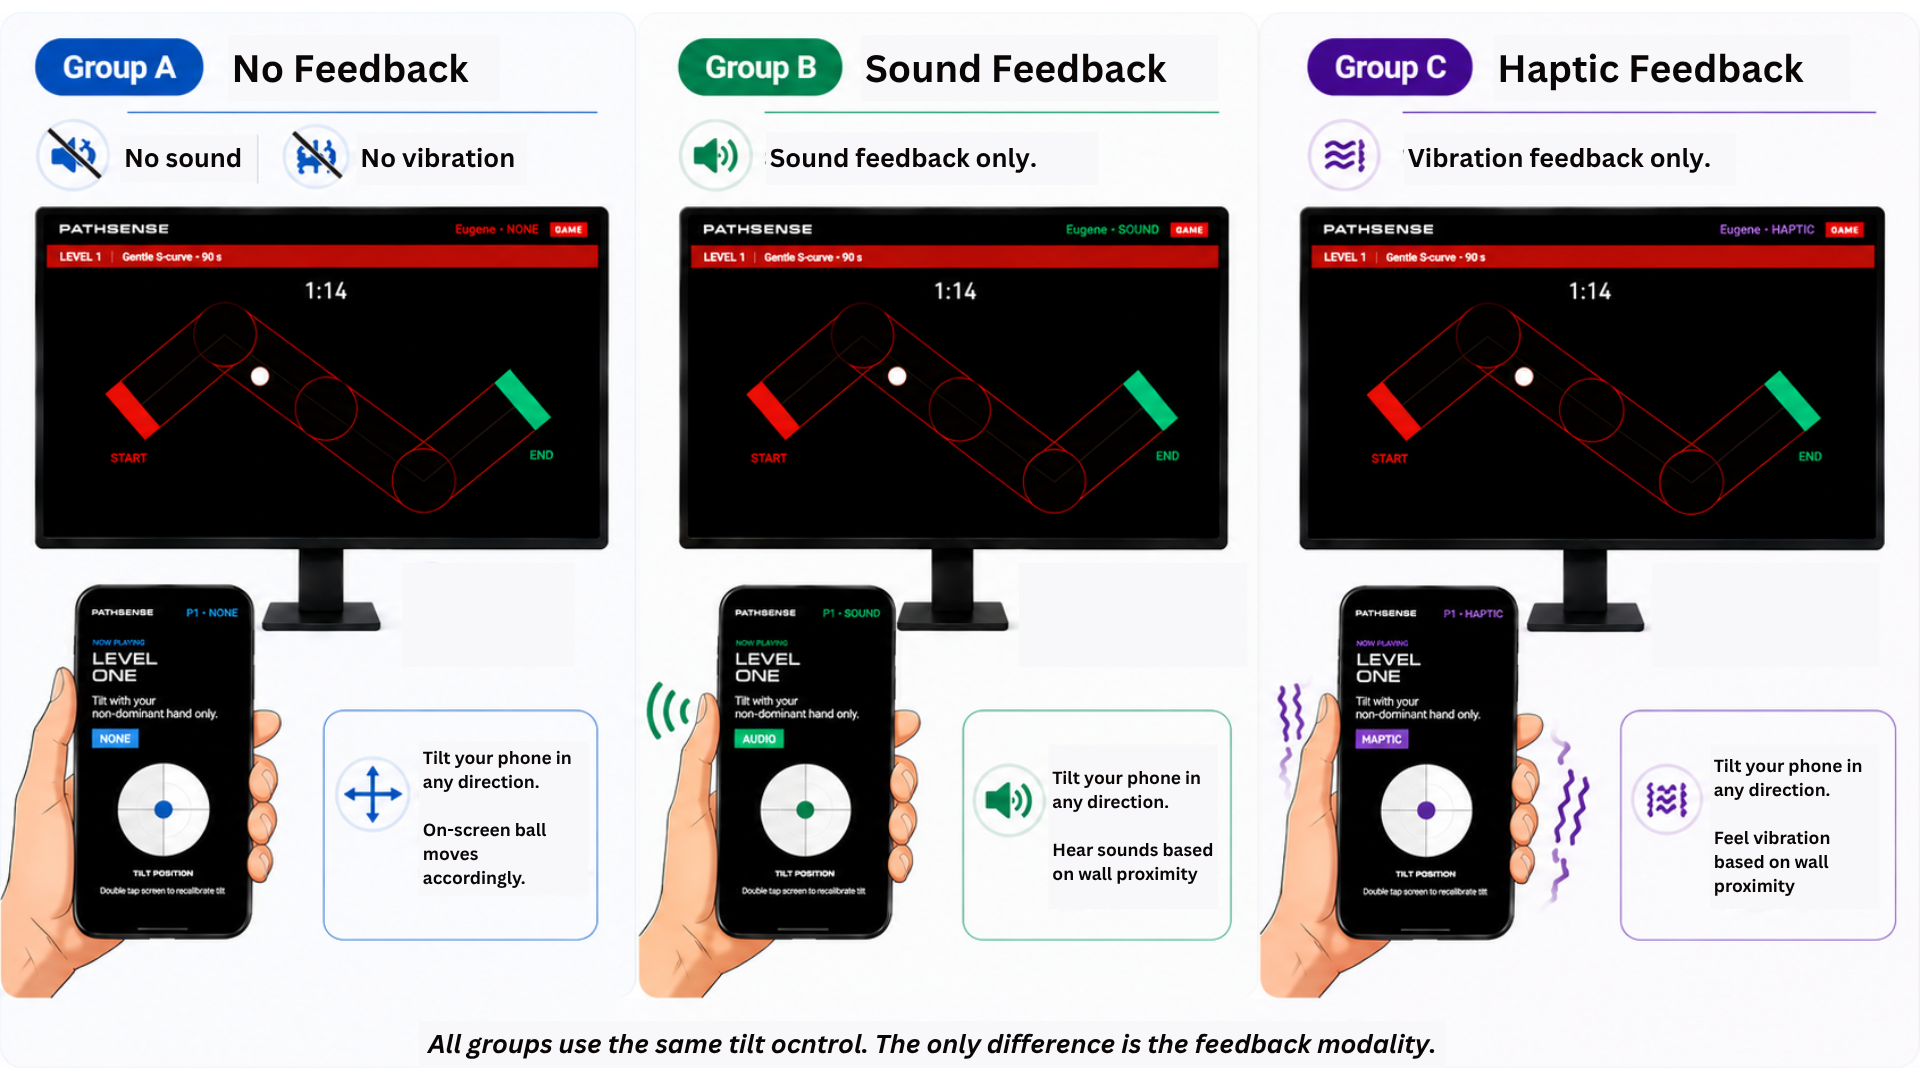
\includegraphics[width=\linewidth]{figure.png}
  \caption{The three between-subjects feedback conditions in PathSense.
    All groups use the same tilt control; the only difference is the feedback modality.}
  \Description{Three-column figure showing the PathSense study conditions:
    Group A (no feedback), Group B (sound feedback), Group C (haptic feedback).
    Each column shows an external monitor with the game display and a hand
    holding the smartphone controller with a tilt-position indicator.}
  \label{fig:teaser}
\end{teaserfigure}

\maketitle

% =========================================================================
\section{Introduction}
% =========================================================================

Tilt-based interfaces appear across gaming controllers, accessibility switches,
and smartphones, and in many of them the non-dominant hand is the one doing
the steering.
It holds the device, absorbs corrections, and keeps things stable, all tasks
that demand real precision from the hand we typically rely on less.
The smartphone is the most familiar example, but the pattern is the same
wherever tilt control falls to the off-hand, something always feels slightly off.
We suggest this reflects a sensory calibration gap, one
that graded feedback from the held device may help close.
When we actively use a tool, the brain extends its spatial self-model to include
the tool's tip~\cite{tools_maravita_2004}.
Maravita and Iriki (2004) demonstrated this in macaque monkeys: after five
minutes of active rake use, bimodal neurons in the intraparietal cortex expanded
their visual receptive fields to span the full length of the tool, as though the
hand itself had elongated, an effect absent during passive grasping.
This mechanism appears to extend to contemporary handheld devices.
Lin et al.\ (2022) showed that smartphones, unlike comparably shaped objects,
may specifically integrate into body schema: across five behavioural experiments,
participants perceived their forearm as longer after imagined smartphone use
and responded faster to smartphone-held hand images than to identically posed
hands holding non-smartphone controls~\cite{smartphone_lin_2022}.
If the held phone is already encoded as a bodily extension, proximity warnings
delivered \emph{through} it may update the user's spatial self-model more
directly than warnings arriving on a separate channel.

The non-dominant hand is a natural target for this kind of augmentation.
Guiard (1987) proposed the kinematic chain model of bimanual action: the
non-dominant limb acts as the \emph{frame-setter}, operating at a coarser
spatial and temporal scale to establish the postural context within which the
dominant hand performs fine-grained movements~\cite{asymmetric_guiard_1987}.
The two limbs also differ in how they process proprioceptive information:
Adamo and Martin (2009) found asymmetric sensory-motor gains at the wrist,
with the non-dominant hand relying more heavily on peripheral proprioceptive
feedback while the dominant hand draws on finer cortical
resolution~\cite{position_adamo_2009}.
Neural data confirm this asymmetry extends to the neural level.
Zabihhosseinian et al.\ (2020) found that after a novel motor tracing task,
the non-dominant hand produced somatosensory evoked potential (SEP) changes
consistent with feedback-based impedance control (a 24\,\% N30 decrease and
a 22\,\% N24 increase), while the dominant hand showed the opposite feedforward
pattern~\cite{differential_zabihhosseinian_2020}.
Augmentation should therefore do more work for the limb that already leans on
incoming sensory signals.

Whether feedback \emph{modality} shapes that benefit is less clear.
Sigrist et al.\ (2013) reviewed over 120 motor learning studies across visual,
auditory, and haptic modalities, concluding that modalities differ substantially
in their mechanisms and design requirements~\cite{augmented_sigrist_2013}.
Haptic feedback operates on the same sensorimotor channel as the task itself:
the hand that acts also receives the warning, creating a more direct coupling
between error signal and corrective movement.
Cuppone et al.\ (2016) provided initial evidence for this: vibrotactile error
feedback during proprioceptive training significantly improved wrist
joint position-sense acuity within three days, whereas training without it did
not, with benefits generalising even to the contralateral
limb~\cite{robotassisted_cuppone_2016}.
Audio warnings, by contrast, are processed on a channel separate from the
executing limb; Sigrist et al.\ (2013) note that while audio can guide
continuous movement effectively, it requires deliberate signal-to-correction
mapping to avoid misinterpretation~\cite{augmented_sigrist_2013}.
Existing evidence for both modalities comes from lab-grade robots and
rehabilitation rigs; whether smartphone-delivered proximity feedback produces
comparable effects in a non-dominant hand tilt task remains untested.

We present \emph{PathSense}, a smartphone tightrope tilt task in which
participants navigate a ball along a narrow pre-designed path using only their
non-dominant hand, receiving graded proximity warnings in one of three
modalities (haptic / audio / none) --- see Figure~\ref{fig:teaser}.
Falls (ball-off-path events) are the primary outcome.
We contribute:
\begin{itemize}
  \item A smartphone-native proximity feedback platform requiring no lab
        apparatus, enabling modality comparison in a standardised, portable
        tilt task
  \item A between-subjects pilot study with a non-dominant-hand constraint
        across three difficulty levels, providing effect size estimates for a
        larger planned follow-up
  \item Preliminary evidence on whether haptic proximity feedback reduces falls
        more than audio or no feedback when the body schema is engaged through
        active single-handed phone use
\end{itemize}

We address the following research questions:

\begin{table}[h]
  \caption{Research Questions}
  \label{tab:rqs}
  \begin{tabular}{p{0.06\linewidth} p{0.86\linewidth}}
    \toprule
    \textbf{RQ} & \textbf{Question} \\
    \midrule
    RQ1\textsuperscript{*} &
      Does continuous proximity-based feedback modality (haptic / audio / none)
      affect fall rate in a tilt-controlled tightrope balance task performed
      with the non-dominant hand? \\[4pt]
    RQ2 &
      Does \emph{any} proximity feedback reduce falls compared to the
      no-feedback condition? \\[4pt]
    RQ3 &
      Which modality (haptic / audio) produces fewer falls? \\[4pt]
    RQ4 &
      Does performance improve across difficulty levels
      (L1\,$\to$\,L2\,$\to$\,L3), and is that improvement
      modality-dependent? \\
    \bottomrule
  \end{tabular}
  \smallskip\par
  \footnotesize\textsuperscript{*}Primary research question.
\end{table}

% =========================================================================
% TODO: add remaining sections
%   \section{Related Work}
%   \section{Study Design}
%   \section{Results}
%   \section{Discussion}
%   \section{Limitations and Future Work}
% =========================================================================

% -------------------------------------------------------------------------
\bibliographystyle{unsrt}
\bibliography{mhci}
% -------------------------------------------------------------------------

\end{document}
